\documentclass[journal]{IEEEtran}

\usepackage{graphicx}  %needed to include png, eps figures
\usepackage{float}  % used to fix location of images i.e.\begin{figure}[H]
\usepackage{amsmath}
\usepackage{gensymb}
\usepackage{hyperref}

\begin{document}

\title{ECSE 444 - Final Report}

\author{Christopher Ghosn, Qihao Wu, Zichen Gao, Nader Akel}

% make the title area
\maketitle

\section{Introduction}
Communication with audio over distances generally takes the form of radios or phones. However, the proliferation of Wi-Fi creates areas where signals do not need to be carried far to go from one device to another. This means that longer-ranged radio signals used in radios and phones are not necessary, keeping those frequencies clear. This requires a pair of devices capable of connecting themselves to a Wi-Fi network so they can transmit audio to each other.

\section{Design Approach}
\subsection{Project Overview}
With the use of two STM32 B-L4S5I-IOT01A development boards, plus peripheral devices such as microphones and speakers, an audio communication link can be established between the two boards over Wi-Fi signals. Voice or audio can be inputted through a microphone, which is transmitted to the board using the DFSDM peripheral. The board can then process the signal in different ways using the CMSIS-DSP (Common Microcontroller Software Interface Standard - Digital Signal Processing), a software library designed for high-performance signal processing on ARM cores. This library is used to process the sound data received by the microphone. Two different implementations using the library are considered: one where the sound is filtered using a built-in CMSIS finite impulse response (FIR) low-pass filter function and the other where a fast Fourier transform (FFT) based compression is used. The former improves quality, while the latter makes the audio take up less space. In both cases, data is then sent via Wi-Fi from one board to the other using the Wi-Fi modules on each board. If the data is compressed, the receiving board first decompresses it before further action. The receiving board then plays the audio through a speaker wired to the board using the Digital-to-Analog module. Figures \ref{Filter} and \ref{Compression} showcase the implementation of our system, both with the low-pass filter and the audio data compression.

\begin{figure}[H]
    \centering
    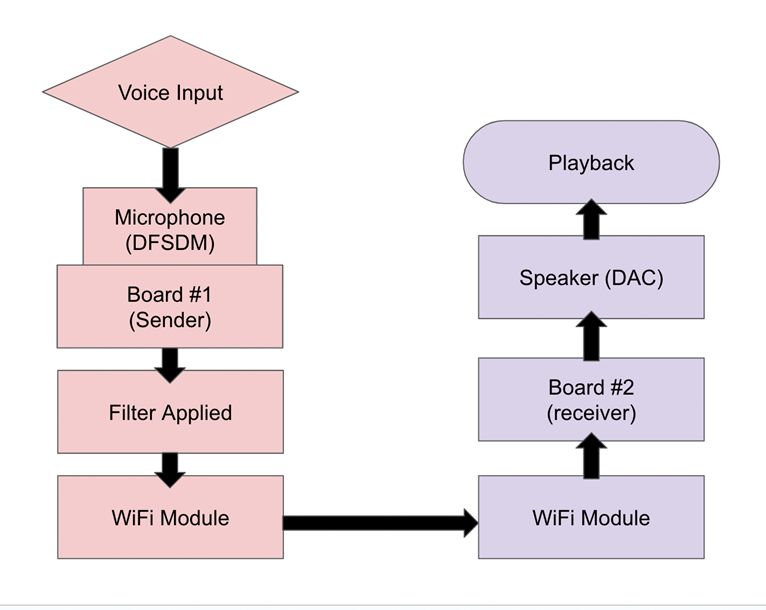
\includegraphics[width=0.7\linewidth]{bibtex/Images/Filter.png}
    \caption{Overview of the system with the low-pass filter}
    \label{Filter}
\end{figure}

\begin{figure}[H]
    \centering
    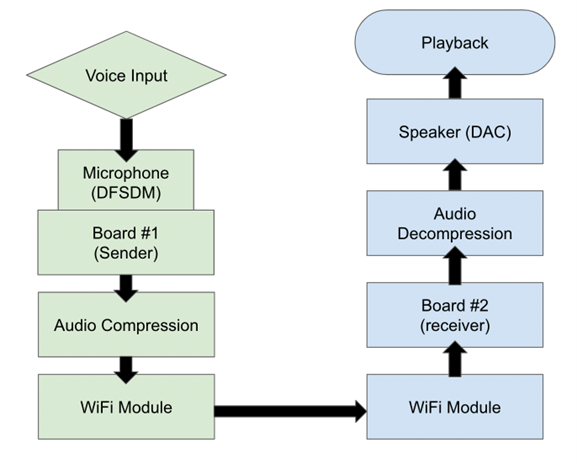
\includegraphics[width=0.7\linewidth]{bibtex/Images/Compression.png}
    \caption{Overview of the system with audio compression}
    \label{Compression}
\end{figure}

\subsection{Software}
The software implementation of the system is divided into two programs: one running on the sender board and one running on the receiver board. The process starts by connecting the two boards to a local Wi-Fi hotspot that we start on a smartphone. The sender board waits for a button press to start recording audio of a fixed length. The low-pass transform or audio data compression algorithm is then applied to the recorded data. After this, it opens a Wi-Fi connection with the other board through the hotspot (the IP address of the receiver board is hard-coded into the program in advance) and starts sending its audio data to the receiver board in several packets wirelessly. The receiver board polls for attempts to connect to it as it waits for data from the sender board. After receiving all the audio recording data, it is decompressed if needed and played on a speaker through the DAC output of the microcontroller.

\subsection{Audio Input and Output}
The audio input and compression subsystem takes in raw audio data from DFSDM microphones on the sending board. On a button press, this subsystem is initiated and the DFSDM microphones start to collect and filter audio data. Using the DMA interface, the function \textit{HAL\_DFSDM\_FilterRegularStart\_DMA()} fills up the buffer, which is 40960 words long, with the word-sized audio samples. The microphone records at a rate of 10 kHz and fills up the buffer in 4.1 seconds. This number was chosen to provide a useful recording length while limiting the memory required to utilize the buffer. Since the Compression Subsystem requires the data to be processed in blocks of size 1024, we chose the microphone buffer to be exactly 40*1024 = 40960, which will imply a total of 40 blocks. An interrupt is raised when the DFSDM has finished collecting data. After the data is successfully sent to the receiving board, the subsystem restarts unless another button press is detected.

The other half of the subsystem uses the Digital-to-Analog converter on the receiving board to convert the data into audio. After receiving all data packets and, if necessary, decompressing the data, the board enters a for loop to cast the transferred buffer into \textit{uint32\_t}. This turns it into the appropriate variable type to be used in a DAC function. After the transformation, \textit{transformBufferToDAC()} is called using the buffer. An analog signal is then sent through the D7 output, which is serially connected via jumper wires to a speaker and a 165\ohm\ resistor, with the GND input acting as the ground. After the electricity reaches the speaker, the sound is played according to the buffer used in the \textit{transformBufferToDAC()} function.

\subsection{Wi-Fi Data Transfer}
The Wi-Fi data transfer subsystem is needed to send data from the sending board to the receiving board wirelessly using an existing Wi-Fi network. The software components include code on the receiving and sending boards, which makes use of an existing Wi-Fi library that controls the onboard Wi-Fi module. The hardware components include the Wi-Fi module itself (es-Wifi).

\vspace{10pt}
\subsubsection{Initiating Wi-Fi}

When both the sending and receiving boards are initiated, they connect to an existing Wi-Fi network via credentials (SSID, Password) which are stored in a C header file. The credentials for the Wi-Fi network are stored in a configuration file (boards.cfg) in the project folder. This configuration file also specifies which board is currently active in the project folder (since both sending\_main.c and receiving\_main.c are in the same folder). We wrote a Python script (config.py) that reads the configuration file and generates header files which specify the Wi-Fi credentials as well as which main file needs to be active. This process of using a script to configure our boards was chosen to minimize time spent manually changing the parameters in each file and to ensure that only one main file is active at a time in the IDE.

Both the sending board and the receiving board begin by connecting to the same Wi-Fi network. First, the function wifi\_start(), which was pre-written in the example Wi-Fi project in the STMCube repository, initiates the Wi-Fi module. Then, both boards call the WIFI\_Connect() function defined in wifi.c (essentially a driver file for the Wi-Fi module) with the credentials stored in the header files. Once the connections have been established, the IP address and other connection details are printed to UART. The IP address of the receiving board needs to be manually copied into the configuration file of the sending board.

\vspace{10pt}
\subsubsection{Connecting boards}
On the sending board, we attempt to connect to the receiving board directly using the IP address stored in the header file. Firstly, a local server is started on the sending board using the function WIFI\_StartServer(), which takes in a “socket” and a “port” argument. It is important to note that the socket and port values need to be kept consistent and different between boards. For our project, we chose (arbitrarily) to have the socket and port settings for the sending board be (1, 10) and for the receiving board (0, 80). Then, we open a connection to the receiving board with the function WIFI\_OpenClientConnection() with the IP address stored in the header file (along with the correct remote socket and port settings). 

\vspace{10pt}
\subsubsection{Sending \& Receiving Data}
In order to send data, the sending board calls the function WIFI\_SendData(), which will send a buffer of characters to a remote socket. The maximum length allowed for a single Wi-Fi data transfer is around 1000 bytes. Before calling this function, the connection between the two boards must be established using WIFI\_OpenClientConnection() and after the data transfer is over, the connection is closed using WIFI\_CloseClientConnection(). The connection is only closed once a response has been received from the receiving board, confirming that the data has been received.
%\vspace{10pt}

The function WIFI\_WaitServerConnection() is being called continuously in a loop as we wait for a connection to open from the sending board. Once a connection is opened, the wifi\_process\_received\_data() function is called, where we then receive the data using WIFI\_ReceiveData(). We then send a confirmation back to the sending board.

\subsection{Compression \& Decompression}
On the sending board, after the data has been put into the buffer by the DFSDM, the buffer is broken up into “blocks” of size 1024. This block size was chosen because the CMSIS fast Fourier transform (FFT) functions only support discrete input sizes which are powers of two (512, 1024, 2048, etc.). Additionally, the maximum data that a Wi-Fi data transfer can support is 1000 bytes. The primary compression function is implemented on the sending board (in \textit{sending\_main.c}) and is called \textit{computeFFTBlock}.

The compression algorithm works on each block of microphone data. The input is first shifted to the right by 8 bits and cast into floating point values. The bit-shifting is done because the DFSDM output only occupies the most significant 24 bits, with the remaining 8 bits representing other information unrelated to the audio signal. Casting the input to floats is necessary, as the CMSIS FFT functions take floating point arrays as input. 

Then, using a CMSIS FFT function, the 1024-point Discrete Fourier Transform (DFT) of the signal is taken. Since the output of the DFT is an array of complex numbers, the output is formatted such that the real and imaginary components of each individual output are placed in succession (see Figure \ref{fig:FFT Output}).

\begin{figure}[H]
    \centering
    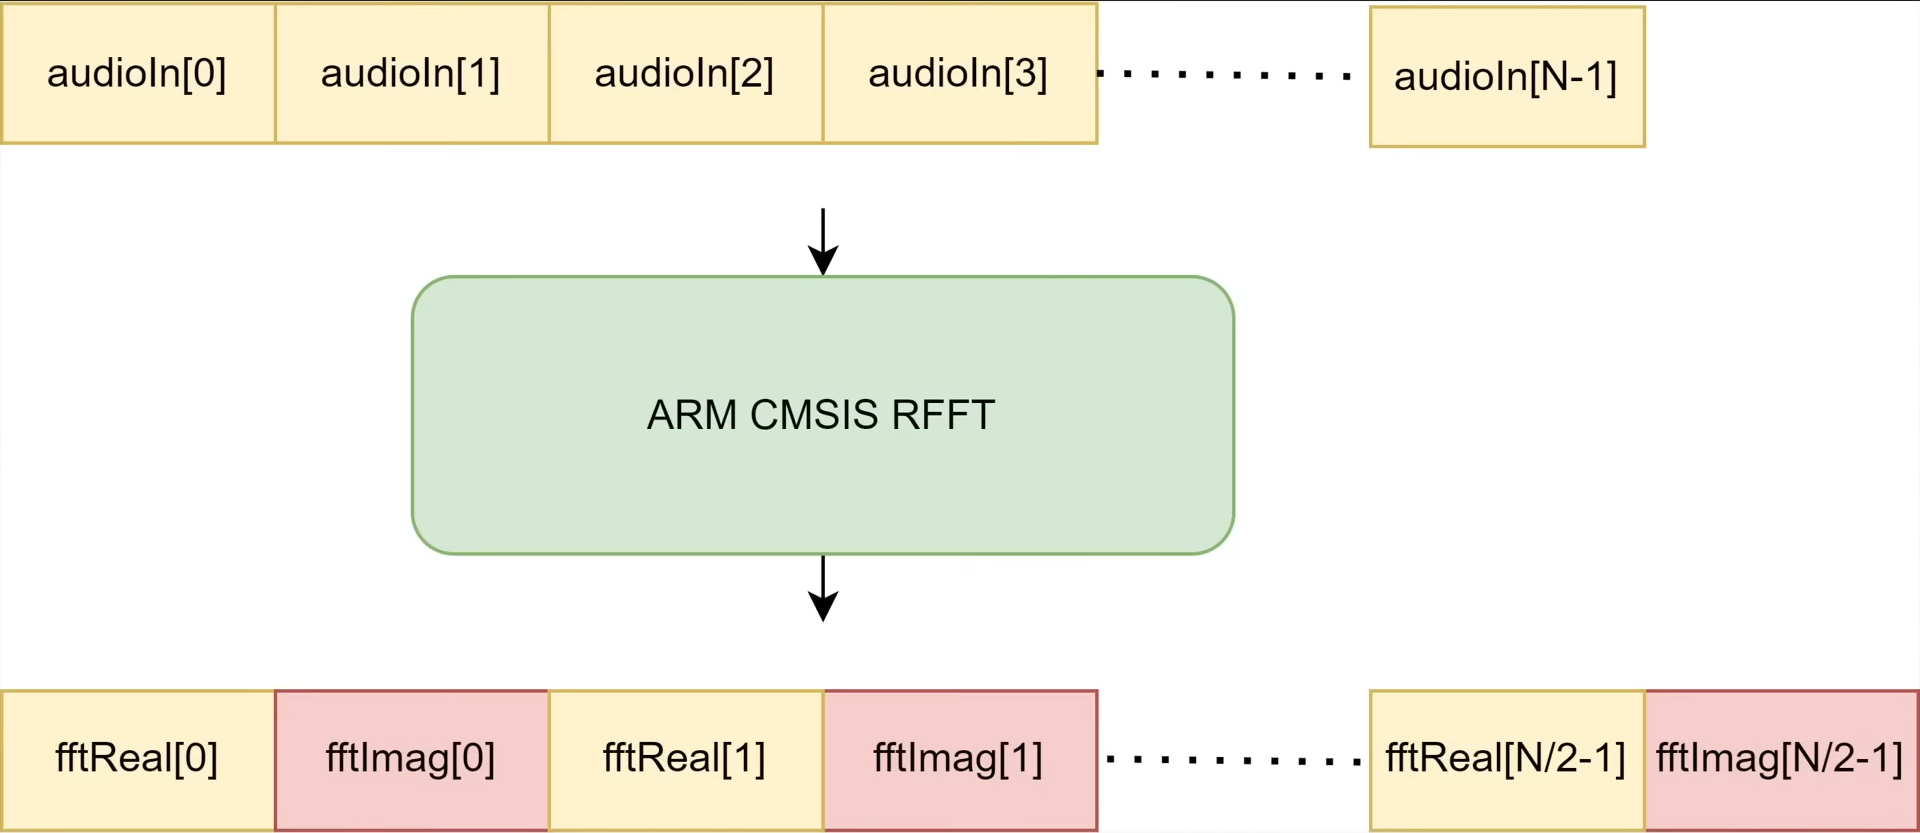
\includegraphics[width=0.8\linewidth]{bibtex/Images/rfft_cmsis_output.png}
    \caption{Output format of the RFFT CMSIS function, taken from \cite{youtube video}}
    \label{fig:FFT Output}
\end{figure}

After taking the DFT, the resulting array is filtered such that components which have a low enough magnitude are set to zero. The cutoff magnitude was experimentally chosen to be 500. Since the Wi-Fi data-sending function \textit{WIFI\_SendData()} only takes in buffers of 8-bit values, we encoded each floating point value in the filtered DCT output array as four individual bytes (characters). Therefore, to completely send each output array would require 1024*4 bytes. However, since we want to compress the data sent over Wi-Fi, we chose to only send the first 512 bytes of the output DFT array. This corresponds to the first 128 floats of the filtered DFT output.

After the data has been sent and received using the Wi-Fi data transfer subsystem, the receiving board implements a decompression algorithm to restore the original audio signal. This decompression algorithm is implemented on the receiving board (receiving\_main.c) and the primary function is called \textit{receiveFFTBlock()}. The received data will be in char format. The first thing to do is to convert it back into floating point values so that the CMSIS FFT functions can perform the inverse FFT algorithm. Then, once the inverse FFT algorithm is performed, the result is cast back into integers and then \textit{transformBufferToDAC()} is called to transform the result into valid 8-bit right-aligned values that can be used for the DAC. 

\subsection{FIR Low-Pass Filter}
The Finite Impulse Response (FIR) low-pass filter is applied on the sending board after the data has been acquired by the DFSDM. The filter coefficients are designed using MATLAB with the fir1() function using a filter order of 2047 and a filtering constraint of 0.1. These numbers are chosen as 2048 would correspond to exactly a twentieth of the length of the buffer, and the filter order needed to be one lower than that value. The cutoff frequency is chosen to be 0.5 kHz, above that of most human voice ranges, and the natural frequency of the microphone is 5 kHz, thus the division giving a filtering constraint of 0.1. After initializing but before utilizing the filter, the buffer goes through a for loop to cast it to float32\_t to work properly with the filtering function. The function arm\_fir\_f32 is then applied to the buffer in a for loop to filter out high-frequency sounds. The sending board then calls transformBufferToDAC() to turn the resulting buffer into valid 8-bit right-aligned values that can be used for the DAC. As can be seen in Figure 1, the filter function is applied before being sent to the Wi-Fi module, but after the sending board receives the data from the microphone. The receiving board requires no additional software, also shown in the figure.

\subsection{Evaluation and Testing Methodology}
Our evaluation and testing methodology was straight forward. Each subsystem was tested using incremental tests / objectives to show proper function. 
\vspace{10pt}

For the Wi-Fi subsystem, we first tested that the example Wi-Fi project provided in the STMCube32 repository worked as intended. The example project was tested successfully, and we were able to observe the web page sent out by the board on a local device (phone). Then, we worked on connecting the two boards to the same Wi-Fi network. After successfully connecting the two boards on the same network, we proceeded to test the various functions in the \textit{wifi.c} library in order to determine how to send data. Once we were able to send data once, we tested sending multiple ``packets'' of data at once. This required opening and closing the connection for each packet sent. Once we tested sending and receiving data multiple times, we determined that our Wi-Fi subsystem was functional.
\vspace{10pt}

For the audio input and output subsystem, we mainly tested the DFSDM and DAC modules after successfully importing them into our project. Especially, since we did not use MXCube (.ioc file) to configure the DFSDM and DAC, we needed to be careful and rigorous with our testing. Indeed, we took multiple samples from the microphone and played them back directly to determine that the DFSDM and DAC were working as intended.
\vspace{10pt}

For the compression and decompression subsystem, we first tested that the \textit{arm\_rfft\_fast\_f32()} function worked properly. We did this by printing out the output of the ARM FFT function for an audio sample taken by the DFSDM, and then copying and pasting the resulting numbers into an Excel spreadsheet. The plot indeed showed a typical DFT distribution. Then, we also tested the inverse FFT function by plotted the results of the inverse FFT and the original signal. An example test is shown in Figure \ref{fig:IFFT_test}, where we see that the inverse FFT plot matches closely with the original signal.
\begin{figure}[H]
    \centering
    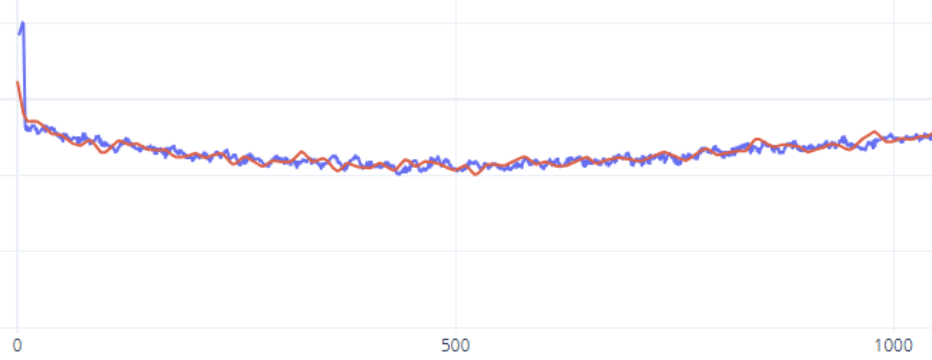
\includegraphics[width=0.8\linewidth]{bibtex//Images/inverse fft.png}
    \caption{Plotting of original audio sample (blue) and inverse FFT (red)}
    \label{fig:IFFT_test}
\end{figure}

After testing the functionality of the ARM FFT functions, we tested the compression and decompression directly on the same board (without sending over Wi-Fi). We did this by playing back the captured audio two times: one where the signal has not gone through the compression and decompression process, and one where the signal goes through the compression and decompression process. We noticed the difference in audio quality between the two playbacks. 
\vspace{10pt}

For the filtering subsystem, we used a similar methodology as the second part of testing the ARM FFT functions, using a single board to play audio two times, one unfiltered playback as a benchmark, and another with the filter on. One button push would start recording and then back the benchmark audio. The next button press plays the audio.


\subsection{Project Progression and Challenges}

We spent the largest amount of our time budget for the project researching the Wi-Fi protocol and how to use the on-board Wi-Fi modules of the development boards. We ended up using an example project provided with STM32CubeIDE as a template for our implementation of the Wi-Fi data transfer. The lack of documentation about the use of Wi-Fi forced us to keep the entire project folder for the program within the example project, as we were not able to find a way to import the Wi-Fi implementation into a proper STM32Cube project. This meant that we did not have access to an IOC file to auto-generate the code necessary to initialize our peripherals, so we had to resort to using Git to figure out how to initialize certain peripherals by checking the changes made to generated code by initializing those peripherals through an IOC file.

\vspace{10pt}
The CMSIS library was also very poorly documented, and we had a hard time figuring out how the provided functions worked, so much so that we had to resort to Fourier transforms to compress the audio data instead of the more efficient discrete cosine transforms. The Fourier transform compression made audio quality take a huge hit, to the point where it was barely understandable. Additionally, the FIR low-pass filter's utility is questionable as the speaker is unable to play high-frequency sounds, which the filter is supposed to reduce.

\vspace{10pt}
We started our project with a 20 kHz audio sample rate for the recording, but we ended up dialing it down to 10 kHz to be able to fit a longer recording length in our buffer at a minimal cost in audio quality. We had originally planned to make it so that both boards could send and receive/play audio, but we did not have enough time to implement this as it would have been very technically challenging.

\section{Optimizations}
We chose to perform compiler-based optimizations to speed up the audio compression and decompression processes. We used ITM debugging to generate data trace calls at the start and end of those processes and be able to measure the time that passed between those calls. We wrote a short Python script (thanks to ChatGPT for help!) that would calculate the average speed of each process from a log file of the SWV Trace Log generated by the IDE.

\vspace{10pt}
We encountered some issues trying to use specific GCC flags to improve performance instead of the \textit{-Ox} presets. We still those issues are bugs in the IDE or come from a lack of understanding of how the compiler works, but none of the GCC flags would yield significant performance improvements. While using heavier presets than \textit{-O0} did result in significant performance improvements, using the flags that were included by those presets and combining them together themselves would not, which was troubling.

\vspace{10pt}
Preset \textit{-O0} ran the forward Fourier transform sequence in about 69132 $\mu$s and the inverse Fourier transform sequence in 51741 $\mu$s. Preset \textit{-O1} performed the forward Fourier transform in 51066 $\mu$s and the inverse Fourier transform in 34254 $\mu$s, which are a 35\% and 51\% speed improvements over preset \textit{-O0}. Preset \textit{-O2} yielded much less significant performance improvements over \textit{-O1} than \textit{-O1} did over \textit{-O0}, by running the forward Fourier transform in 50821 $\mu$s and the inverse Fourier transform in 33406 $\mu$s, which are only 0.4\% and 2.5\% improvements over preset \textit{-O1}. Finally, presets \textit{-O3} and \textit{-Ofast} yielded very negligible performance improvements, to the point that they could be considered to perform within the margin of error of \textit{-O2}.

\section{Conclusion}

The project yielded two separate systems that both recorded a four-second audio clip on one STM32 B-L4S5I-IOT01A development board, sent it to a second board over an existing Wi-Fi network, and then played it on a speaker. The difference between the systems is that one compresses the audio with a 2-to-1 ratio, thus reducing the bandwidth required by half, while the other features an FIR low-pass filter, filtering out higher-frequency sounds. 

Looking back, there are a few things that could have been done differently to save us time. One example would be the fact that we did not have an IOC file. This made it very hard and time-consuming to configure the different components on the sender and receiver boards. In retrospect, research on the different CMSIS functions could have been done near the beginning of the project. Something else that we could have done to save time is to work on the different parts of the subsystems simultaneously and have a predetermined testing method that’s easily quantifiable from the start of the project. 

\vspace{10pt}
A demo of the project can be found here: \url{https://www.youtube.com/watch?v=PtOjv1w0G0o}

\begin{thebibliography}{9}
\bibitem{youtube video}
Phil's Lab. "STM32 Fast Fourier Transform (CMSIS DSP FFT) - Phil's Lab \#111," YouTube, June 20, 2023.
Available: \url{https://www.youtube.com/watch?v=d1KvgOwWvkM&ab_channel=Phil%E2%80%99sLab}. [Accessed: Dec 5, 2023].
\end{thebibliography}
\end{document}